\documentclass[12pt,a4paper]{article}

\usepackage{kotex}
\usepackage{amsmath,amssymb,amsfonts}
\usepackage{graphicx}
\usepackage{textcomp}
\usepackage{xcolor}
\usepackage{booktabs}
\usepackage{multirow}
\usepackage{url}
\usepackage{array}
\usepackage{balance}
\graphicspath{{../../figures/}}

\begin{document}

\title{TA-BRPL 연구노트 v0.3.1\\
Blackhole + Sinkhole 복합 공격 환경에서의\\
Trust-Aware Backpressure RPL 구현 및 초기 결과}

\author{연구노트 v0.3.1 --- Internal Draft\\최종 수정: 2026-03-18}

\maketitle

% ============================================================
\begin{abstract}
% ============================================================
본 문서는 TA-BRPL(Trust-Aware Backpressure RPL)의 현재 구현 상태와 최신 실험 결과를
통합 정리한 연구노트이다. 대상 환경은 Contiki-NG/Cooja 기반의 $6\times6$ GRID 토폴로지
(총 36개 노드, 30개 random seed)이며, 3개의 blackhole 공격자(node 2, 3, 4)와
1개의 sinkhole 공격자(node 18)가 동시에 동작하는 복합 공격 시나리오를 가정한다.

TA-BRPL은 BRPL의 backpressure 기반 경로 선택 능력을 유지하면서,
3성분 on-node trust 모델($T_\text{fwd}$, $T_\text{ctrl}$, $T_\text{hon}$)을
BRPL objective function에 직접 결합한다. 전체 30-seed 실험에서 TA-BRPL은
during-attack PDR \textbf{0.9077}, recovery PDR \textbf{0.9593}을 기록하여,
RPL(0.8759/0.8754), BRPL(0.8508/0.8399), SMTrust(0.8701/0.8649) 대비
더 높은 공격 복원력을 보였다.

본 문서는 설계 의도, 전체 구현 구조, 실험 설정, 30-seed 기본 결과,
EWMA/임계값 민감도 분석, 성분 절제 실험, 혼잡--공격 분리 실험,
오탐 실험, 손실률 로버스트니스, 그리고 현재 한계와 후속 과제를 정리한다.
\end{abstract}

\textbf{키워드:} IoT, LLN, RPL, BRPL, Trust Management, Blackhole, Sinkhole,
Selective Forwarding, Cooja, Contiki-NG

% ============================================================
\section{연구 목표}
% ============================================================

본 연구의 목적은 LLN(Low-power and Lossy Network) 환경에서 다음의 두 가지 상충되는 요구를
동시에 만족시키는 것이다. 첫째, BRPL이 제공하는 backpressure 기반 혼잡 인식 라우팅
능력을 유지한다. 둘째, blackhole(선택적 패킷 드롭)과 sinkhole(rank 조작)과 같은
insider routing attack에 대해 노드 내 자율적 복원력을 확보한다.

기존 접근의 한계는 크게 두 가지다. 첫째, 단순 forwarding rate 기반 감시는
혼잡과 공격을 구분하지 못한다. 즉, 정직하지만 혼잡한 노드와 의도적으로 패킷을
드롭하는 공격자는 모두 forwarding rate 하락을 유발한다. 둘째, SMTrust와 같이
weighted-sum trust를 MRHOF 위에 얹는 구조는 정적 환경에서 일부 가중치 성분이
상수처럼 고정되어 trust floor가 탐지 임계값 이상에 묶이는 구조적 한계를 가진다
(Section~\ref{sec:smtrust} 참조).

TA-BRPL의 핵심 가설은 다음과 같다.
\begin{itemize}
  \item $T_\text{fwd}$: 수동 도청(passive overhearing) 기반 forwarding success rate로 blackhole을 탐지한다.
  \item $T_\text{ctrl}$: DIO rank/version 이상 징후를 활용해 sinkhole을 탐지한다.
  \item $T_\text{hon}$: 큐 광고값과 로컬 추정치의 교차 검증을 통해 혼잡과 공격을 분리한다.
  \item 세 성분의 가중 기하평균을 trust로 집계하고 이를 BRPL cost function에 직접 결합함으로써,
  공격자 parent가 점진적으로 배제되도록 한다.
\end{itemize}

% ============================================================
\section{전체 시스템 구조}
% ============================================================

\subsection{계층 구조}

TA-BRPL은 Contiki-NG의 RPL-Classic 라우팅 스택 위에서 동작한다.
핵심 모듈은 \texttt{ta-brpl-trust.c/h}(trust 엔진, 약 850 LoC)이며,
\texttt{rpl-brpl.c}의 objective function에 C weak-symbol 오버라이드를 통해
결합된다. 이 설계는 TA-BRPL을 컴파일에서 제거하더라도 BRPL/RPL의
원본 소스를 직접 수정할 필요가 없음을 의미한다.

네트워크 스택에서 trust 엔진으로 입력되는 훅은 다음 세 가지다.
\begin{enumerate}
  \item \textbf{IP input hook} (\texttt{NETSTACK\_CONF\_IP\_INPUT\_CALLBACK}):  
  릴레이 unicast 패킷을 감지하여 $T_\text{fwd}$ 관찰 이벤트를 공급하고,
  DIO ICMPv6 메시지를 파싱하여 $T_\text{ctrl}$ 이상 지표를 갱신한다.
  \item \textbf{BRPL queue callback}:  
  이웃 노드의 큐 광고값($Q_\text{adv}$, $Q_\text{max}$)을 전달하여
  $T_\text{hon}$ 계산에 사용한다.
  \item \textbf{RPL parent-change callback}
  (\texttt{RPL\_CALLBACK\_PARENT\_SWITCH}):  
  preferred parent 교체 시 \texttt{current\_parent\_id}와 escape 타이머를 갱신한다.
  이 훅이 없으면 escape 메커니즘은 발동하지 않는다.
\end{enumerate}

trust 엔진에서 BRPL 측으로 전달되는 출력은 다음의 세 weak-symbol 함수로 제공된다.
\begin{itemize}
  \item \texttt{brpl\_trust\_get(node\_id)}: trust 값 [0, 1000] 반환
  \item \texttt{brpl\_penalty\_scale\_get(node\_id)}: 지속 패널티 배율 반환
  \item \texttt{brpl\_escape\_mode\_get(node\_id)}: 탈출 모드 플래그 반환
\end{itemize}

\subsection{파라미터 단일 소스}

모든 tunable parameter는 \texttt{project-conf.h}의 C 매크로로 정의된다.
각 프로토콜 변형의 \texttt{Makefile.*}은 모드 플래그만 설정하며,
임계값 및 $\lambda$ 값은 모두 \texttt{project-conf.h}에서만 관리된다.
민감도 실험은 컴파일러 커맨드라인에서 특정 매크로만 오버라이드하는 방식으로 수행한다.

% ============================================================
\section{Trust 모델 상세}
% ============================================================

\subsection{$T_\text{fwd}$: Forwarding Trust}

$T_\text{fwd}$는 이웃 $j$가 패킷을 얼마나 신뢰성 있게 중계하는지를
측정하는 성분이다. 노드 $i$는 이웃 $j$를 통해 패킷을 전송할 때마다
카운터 $S_{ij}$를 증가시키고, $j$가 임의의 unicast 패킷을 IP 레이어에서
릴레이하는 것을 도청할 때마다 $F_{ij}$를 증가시킨다.
초기 trust가 과도하게 0 또는 1로 치우치지 않도록 Laplace smoothing
파라미터 $(\alpha,\beta)$를 적용하여 초기값을 0.5 근방으로 유지한다.
\begin{equation}
  T_\text{fwd}(i,j) = \frac{F_{ij} + \alpha}{S_{ij} + \alpha + \beta}.
  \label{eq:tfwd}
\end{equation}

카운터는 150초 업데이트 주기마다 \textbf{우측 비트시프트(halving)}로 감쇠된다.
여기서 리셋 대신 halving을 사용하는 이유는, 완전 리셋을 사용할 경우
공격자가 잠시 정상적으로 패킷을 전달하는 것만으로 trust가 다시 0.5 수준으로
중립화되는 문제가 발생하기 때문이다.

\subsection{$T_\text{ctrl}$: Control-Plane Trust}

$T_\text{ctrl}$은 제어 평면 이상을 세 가지 지표로 탐지한다.

\textbf{Rank 이상 $A_\text{rank}$}: DIO에 포함된 rank가 root rank보다 낮으면
물리적으로 불가능한 상태이므로 즉시 최대 이상으로 처리한다.
또한 과도한 rank 변동은 hysteresis 기준을 초과한 변화 횟수로 누적한다.

\textbf{DIO 빈도 이상 $A_\text{DIO}$}: trickle 타이머 기준의 기대 전송률 대비
과도하게 많은 DIO 전송 횟수를 누적하여 DIO suppression/flooding 이상을 탐지한다.

\textbf{Version 이상 $A_\text{ver}$}: root에서 전파되지 않은 RPL version 번호의 증가는
DODAG 강제 리셋을 유발하는 version attack의 신호로 해석한다.

세 지표를 가중합하여 제어 평면 이상 점수를 계산하고 이를 trust로 변환한다.
\begin{equation}
  A_{ij} = \frac{w_1 A_\text{rank} + w_2 A_\text{DIO} + w_3 A_\text{ver}}{10},\quad
  T_\text{ctrl}(i,j) = 1 - A_{ij}.
\end{equation}
기본 가중치는 $w_1=5$, $w_2=3$, $w_3=2$이다.

\subsection{$T_\text{hon}$: Congestion-Honesty Trust}

$T_\text{hon}$은 이웃 $j$가 자신의 큐 상태를 정직하게 광고하는지를
검증하는 성분이다.
\begin{equation}
  T_\text{hon}(i,j) = 1 - \min\!\left(1,\; \frac{|Q_\text{adv} - Q_\text{est}|}{Q_\text{max}}\right).
\end{equation}

여기서 $Q_\text{adv}$는 이웃 $j$가 BRPL 비콘에 실어 보낸 큐 점유율이고,
$Q_\text{est}$는 노드 $i$가 자신의 로컬 상태로부터 추정한
이웃 $j$의 예상 부하다. 정직하게 혼잡한 노드는 대체로
$Q_\text{adv} \approx Q_\text{est}$를 만족하므로 $T_\text{hon} \approx 1.0$을 유지한다.
반면 공격자가 큐 상태를 실제보다 낮게 광고하면 두 값의 차이가 커지고,
그 결과 $T_\text{hon}$이 하락한다.

이 성분은 ``혼잡으로 인해 forwarding rate가 낮아진 정직한 노드''와
``의도적으로 패킷을 드롭하는 공격자''를 구분하기 위해 필요하다.

\subsection{가중 기하평균 집계}

세 trust 성분은 다음과 같이 가중 기하평균으로 결합된다.
\begin{equation}
  \tilde{T}(i,j) =
  T_\text{fwd}^{w_f/W}
  \cdot
  T_\text{ctrl}^{w_c/W}
  \cdot
  T_\text{hon}^{w_h/W},
\end{equation}
여기서 $W = w_f + w_c + w_h = 10$이며, 기본 가중치 벡터는
$(w_f, w_c, w_h) = (5, 3, 2)$이다.

기하평균을 사용하는 이유는 어느 한 성분이라도 0에 가까워지면
전체 trust가 크게 하락하기 때문에, 공격자가 특정 단일 지표만 조작해서
높은 trust를 유지하기 어렵기 때문이다.

\subsection{비대칭 EWMA 업데이트}

150초마다 다음 점화식으로 per-neighbor trust를 업데이트한다.
\begin{equation}
  T_{ij}(t+1) = \lambda(t)\, T_{ij}(t) + (1-\lambda(t))\, \tilde{T}_{ij},
\end{equation}
\begin{equation}
  \lambda(t) =
  \begin{cases}
    \lambda_\downarrow = 0.5, & \tilde{T}_{ij} < T_{ij}(t)\quad \text{(신뢰 하락 시)} \\
    \lambda_\uparrow   = 0.7, & \text{otherwise}\quad \text{(신뢰 유지/회복 시).}
  \end{cases}
\end{equation}

$\lambda_\downarrow=0.5$는 공격 직후 trust가 빠르게 하락하도록 허용하고,
$\lambda_\uparrow=0.7$은 회복 속도를 의도적으로 늦춰,
공격자가 잠시 정상 동작을 보이며 trust를 회복하는 on-off 전략에 대응한다.

모든 연산은 고정소수점(정수 범위 $[0,1000]$, 해상도 1/1000)으로 수행된다.
기하평균 계산에 필요한 지수 연산은 추후 lookup table 기반으로 대체 가능하다.

\subsection{3단계 임계값 정책}

\begin{table}[t]
  \centering
  \caption{TA-BRPL trust tier 정의}
  \label{tab:thresholds}
  \begin{tabular}{lllp{3.2cm}}
    \toprule
    Tier & 범위 & 상태 & BRPL 효과 \\
    \midrule
    Normal    & $T \ge 700$     & NORMAL      & 패널티 없음 \\
    Suspect   & $450 \le T < 700$ & SUSPECT   & cost 배율 패널티 적용 \\
    Untrusted & $250 \le T < 450$ & UNTRUSTED & parent 후보 제외 \\
    Blacklist & $T < 250$       & BLACKLISTED & 120초 하드 격리 \\
    \bottomrule
  \end{tabular}
\end{table}

parent 선택 시 이웃 $j$의 BRPL routing cost는 다음과 같이 조정된다.
\begin{equation}
  \text{cost}'(j) = \text{cost}(j) \times \frac{P_s(j)}{1000},
\end{equation}
여기서 $P_s(j)$는 Normal 노드에서는 1000(즉, 효과 없음)이며,
Suspect 노드에서는 상황에 따라 700$\sim$1700 범위의 가변 패널티를 갖는다.
Blacklisted 노드는 parent 후보 집합에서 완전히 제외된다.

\subsection{지속 패널티와 탈출 메커니즘}

현재 preferred parent가 공격자인 경우, RPL 자체의 parent-change hysteresis가
전환을 지연시키거나 막을 수 있다. TA-BRPL은 이를 극복하기 위해 두 가지 메커니즘을 둔다.

\textbf{Attack persistence penalty}: preferred parent의 trust가
$\tau_\text{warn}=700$ 미만인 상태가 지속되면, 매 120초 창마다
패널티 배율에 250을 가산한다(최대 2600).

\textbf{Escape mode}: preferred parent의 trust가 $\tau_\text{warn}$ 미만인 상태가
180초 이상 지속되면 escape mode를 활성화한다.
이 모드에서는 현재 parent에 대한 hysteresis가 해제되고,
추가 패널티 배율 3200이 적용되어 metric 차이와 무관하게 parent 교체가 강제된다.

격리 해제 후에는 trust를 $\tau_\text{join}=450$으로 복원하고,
패널티 배율을 120초 동안 $1.6\times \rightarrow 1.0\times$로 선형 감쇠시키며,
재드롭 감시 플래그를 활성화하여 공격이 재개될 경우 즉시 재격리한다.

% ============================================================
\section{SMTrust 구현 상태 및 구조적 한계}
\label{sec:smtrust}
% ============================================================

\subsection{현재 구현}

SMTrust는 ``RPL + trust-aware parent filtering'' 구조로 구현되어 있다.
기반 라우팅은 MRHOF이며, parent 선택 시 다음의 두 단계를 거친다.
\begin{enumerate}
  \item trust class $t_1$/$t_2$ 노드를 후보에서 제외한다 (threshold 0.46).
  \item near-tie 상황에서는 $t_4$/$t_5$ 노드를 $t_3$ 노드보다 우선한다.
\end{enumerate}

Trust index는 다음과 같은 6개 성분의 가중합으로 계산된다.
\begin{equation}
  \text{TI} = 0.25\,\text{TMSR} + 0.15\,\text{TM}_{H_0}
             + 0.15\,\text{TMEL} + 0.20\,\text{TMLLS}
             + 0.15\,\text{TMMobility} + 0.10\,\text{TMRT}.
\end{equation}

\subsection{구조적 한계: TI Floor}

현재 실험 환경은 정적 $6\times6$ GRID 토폴로지이므로, 두 성분이 사실상 상수로 고정된다.
\begin{itemize}
  \item \textbf{TMEL} (가중치 0.15): 이웃의 실제 잔여 에너지가 아니라
  로컬 Energest 추정치를 사용하므로 환경 전반에서 거의 상수 $\approx 0.50$로 유지된다.
  \item \textbf{TMMobility} (가중치 0.15): 정적 토폴로지이므로 $=1.00$으로 고정된다.
\end{itemize}

즉, 총 결합 가중치 0.30이 변별력을 갖지 못한 채 상수처럼 작용한다.
$\text{TMSR}=0$인 완전 blackhole 극단 시나리오를 가정하면 TI의 최솟값은 다음과 같다.
\begin{align}
  \text{TI}_\text{min}
  &= 0 \cdot 0.25 + 0.50 \cdot 0.15 + 0.50 \cdot 0.15 \notag\\
  &\quad + 0.57 \cdot 0.20 + 1.00 \cdot 0.15 + 0.50 \cdot 0.10 \notag\\
  &= 0.464 > 0.460 \quad \text{(필터링 임계값)}.
\end{align}
30-seed 실측 최솟값 역시 $\text{TI}_\text{min}=0.489$였다.

따라서 공격자 노드는 아무리 패킷을 드롭하더라도 TI가 임계값 아래로
충분히 내려가지 않아 parent 후보 집합에서 제거되지 않는다.

이는 단순 구현 버그라기보다, \textbf{구현--환경 불일치}
(implementation-environment mismatch)로 해석하는 것이 더 적절하다.
즉, 실제 이동성이 존재하거나 에너지 정보 교환이 가능한 환경에서는
TMMobility와 TMEL이 변별력을 가질 수 있으나, 현재 실험 환경에서는 그렇지 않다.

% ============================================================
\section{실험 설정}
% ============================================================

\subsection{토폴로지와 노드 역할}

실험 토폴로지는 $6\times6$ GRID, 총 36개 노드이며,
노드 간 간격은 40\,m, 전파 모델은 UDGM
(\texttt{tx\_range=50\,m}, \texttt{success\_ratio=1.0})를 사용하였다.

\begin{itemize}
  \item \textbf{Node 1}: DODAG root (border router)
  \item \textbf{Node 2, 3, 4}: Blackhole 공격자. 350초 이후 전달해야 할 UDP 패킷을 100\% 드롭하며, DIO/routing 동작은 정상적으로 유지
  \item \textbf{Node 18}: Sinkhole 공격자. DIO에 rank$+1$을 광고하여 인근 노드를 유인하고, 유입된 트래픽은 드롭
  \item \textbf{나머지 31개 노드}: Sender. 30초마다 root에 UDP 패킷을 전송
\end{itemize}

\begin{figure}[t]
  \centering
  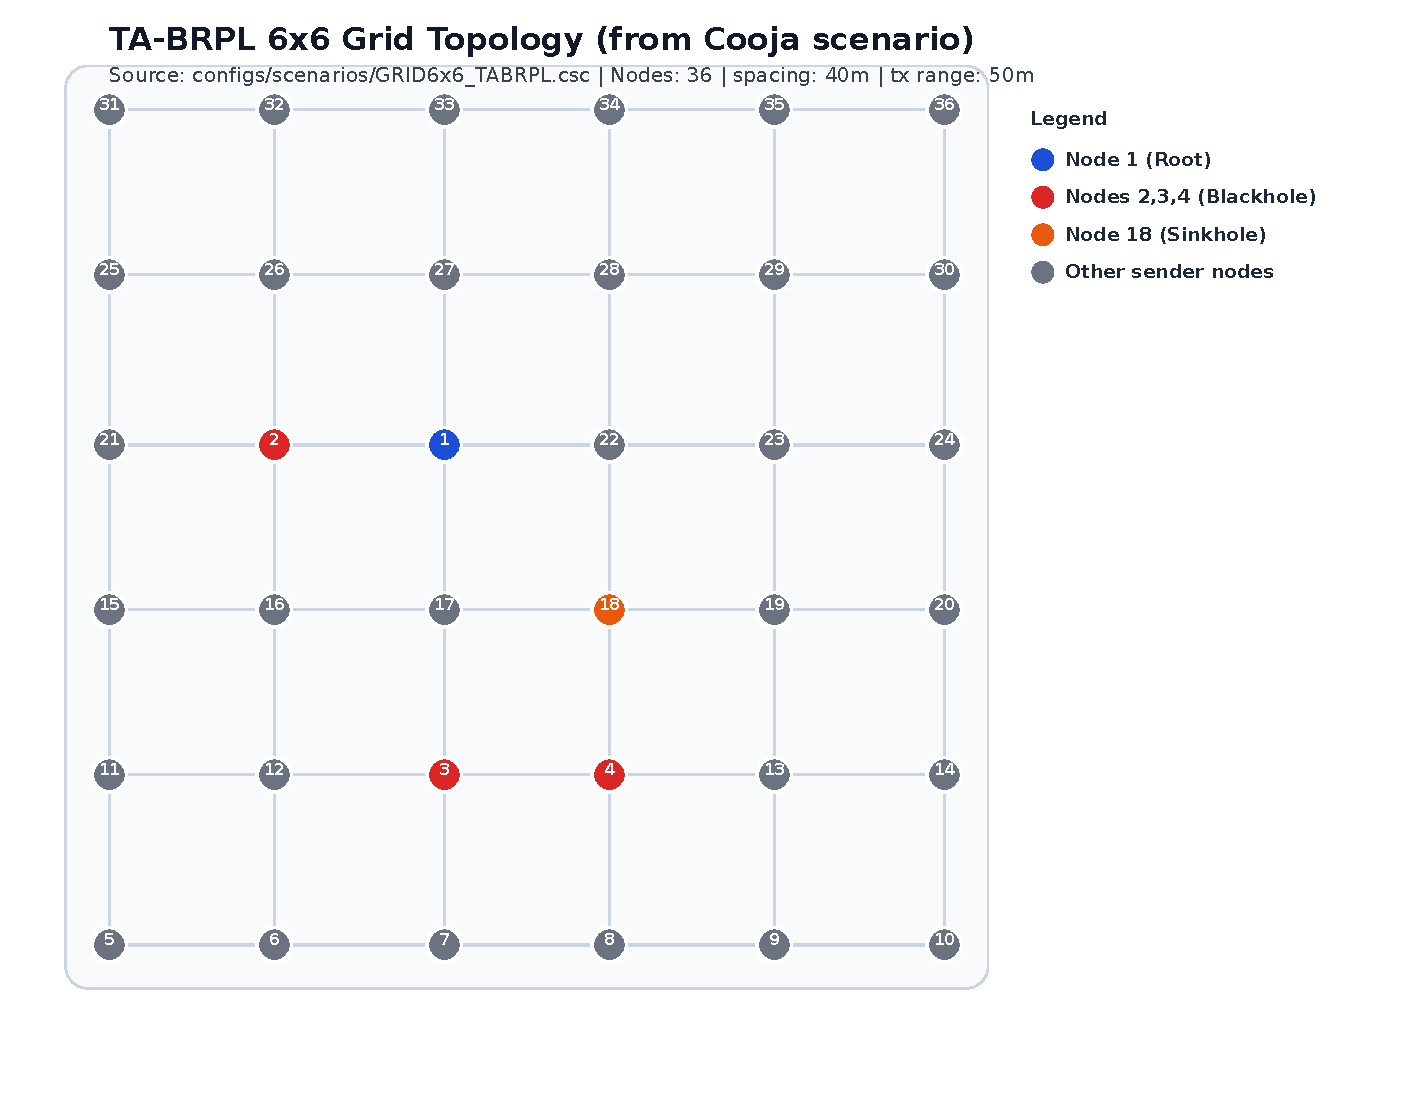
\includegraphics[width=0.95\linewidth]{fig0_topology_grid6x6.pdf}
  \caption{실험 토폴로지($6\times6$ GRID). Node 1은 root, Node 2/3/4는 blackhole,
  Node 18은 sinkhole, 나머지 노드는 sender이다.}
  \label{fig:topology_grid}
\end{figure}

\subsection{실험 타임라인}

\begin{itemize}
  \item $[0,150)$초: Warm-up. DODAG 형성 및 초기 수렴 단계, 통계 미수집
  \item $[150,350)$초: Pre-attack. 정상 동작 구간, 기준 PDR 측정
  \item $[200,300)$초: \textit{(pre-attack 내부)} 합성 혼잡 버스트.
  root 인접 5개 노드가 15초 주기로 추가 송신하여 큐 포화를 유도하고,
  $T_\text{hon}$의 혼잡 인식 능력을 검증
  \item $[350,650)$초: During attack. 공격자 활성화, 주요 PDR 측정 구간
  \item $[650,900)$초: Recovery. 공격자는 계속 활성 상태를 유지하나,
  trust 기반 우회가 수렴한 이후의 PDR 측정
\end{itemize}

전체 시뮬레이션 시간은 900초이며, random seed는 총 30개를 사용하였다.
통계 검정은 Wilcoxon rank-sum test(비모수, Bonferroni 보정)를 적용하였다.

\subsection{비교 프로토콜}

\begin{itemize}
  \item \textbf{RPL}: RPL-Classic + MRHOF/ETX, trust 비활성
  \item \textbf{BRPL}: BRPL + queue-aware cost, trust 비활성
  \item \textbf{SMTrust}: RPL-Classic MRHOF + 6성분 trust filtering
  \item \textbf{TA-BRPL}: 제안 프로토콜
\end{itemize}

% ============================================================
\section{전체 30-Seed 기본 결과}
\label{sec:main}
% ============================================================

Table~\ref{tab:main_pdr}는 4개 프로토콜의 phase별 평균 PDR을 보여준다.

\begin{table}[t]
  \centering
  \caption{Phase별 평균 PDR (30 seeds)}
  \label{tab:main_pdr}
  \begin{tabular}{lrrr}
    \toprule
    프로토콜 & Pre-attack & During attack & Recovery \\
    \midrule
    TA-BRPL  & 0.9993 & \textbf{0.9077} & \textbf{0.9593} \\
    RPL      & 1.0000 & 0.8759 & 0.8754 \\
    SMTrust  & 0.9998 & 0.8701 & 0.8649 \\
    BRPL     & 0.9999 & 0.8508 & 0.8399 \\
    \bottomrule
  \end{tabular}
\end{table}

\textbf{TA-BRPL vs. RPL}: during에서 $+3.2$\,pp, recovery에서 $+8.4$\,pp 개선되었다.  
\textbf{TA-BRPL vs. BRPL}: during에서 $+5.7$\,pp, recovery에서 $+11.9$\,pp 개선되었다.  
모든 pairwise 비교에서 Wilcoxon 검정 결과는 $p < 0.001$이었다.

\begin{figure}[t]
  \centering
  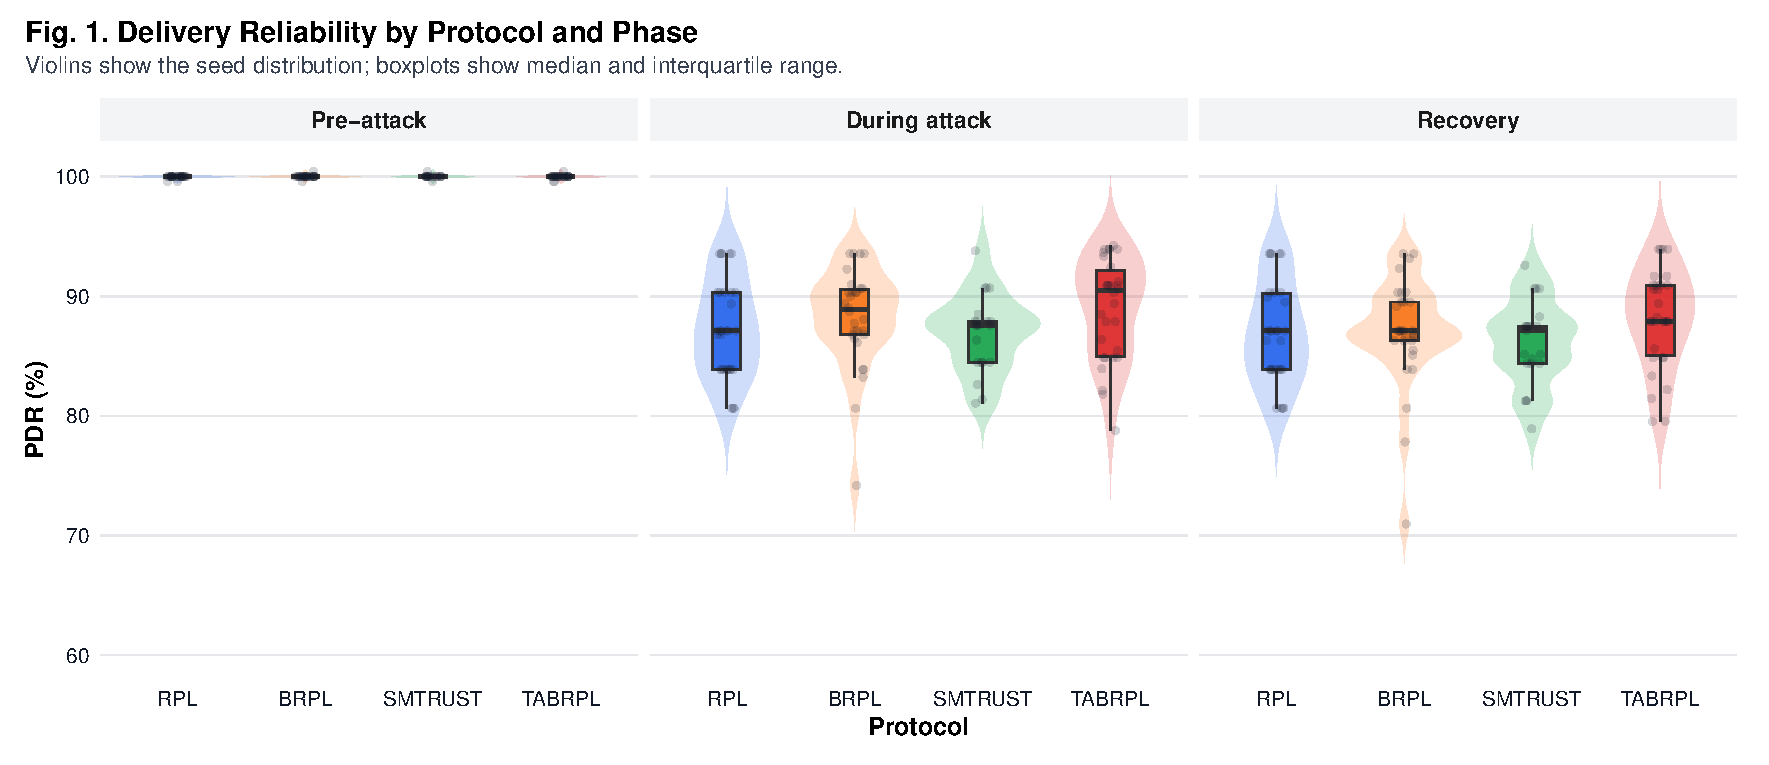
\includegraphics[width=\linewidth]{fig1_pdr_phases.pdf}
  \caption{Phase별 PDR 비교 (30 seeds). 각 박스는 25--75 백분위수, 수염은 10--90 백분위수를 나타낸다.
  TA-BRPL은 during-attack과 recovery 두 구간 모두에서 가장 높은 PDR을 달성한다.}
  \label{fig:pdr_phases}
\end{figure}

\begin{figure}[t]
  \centering
  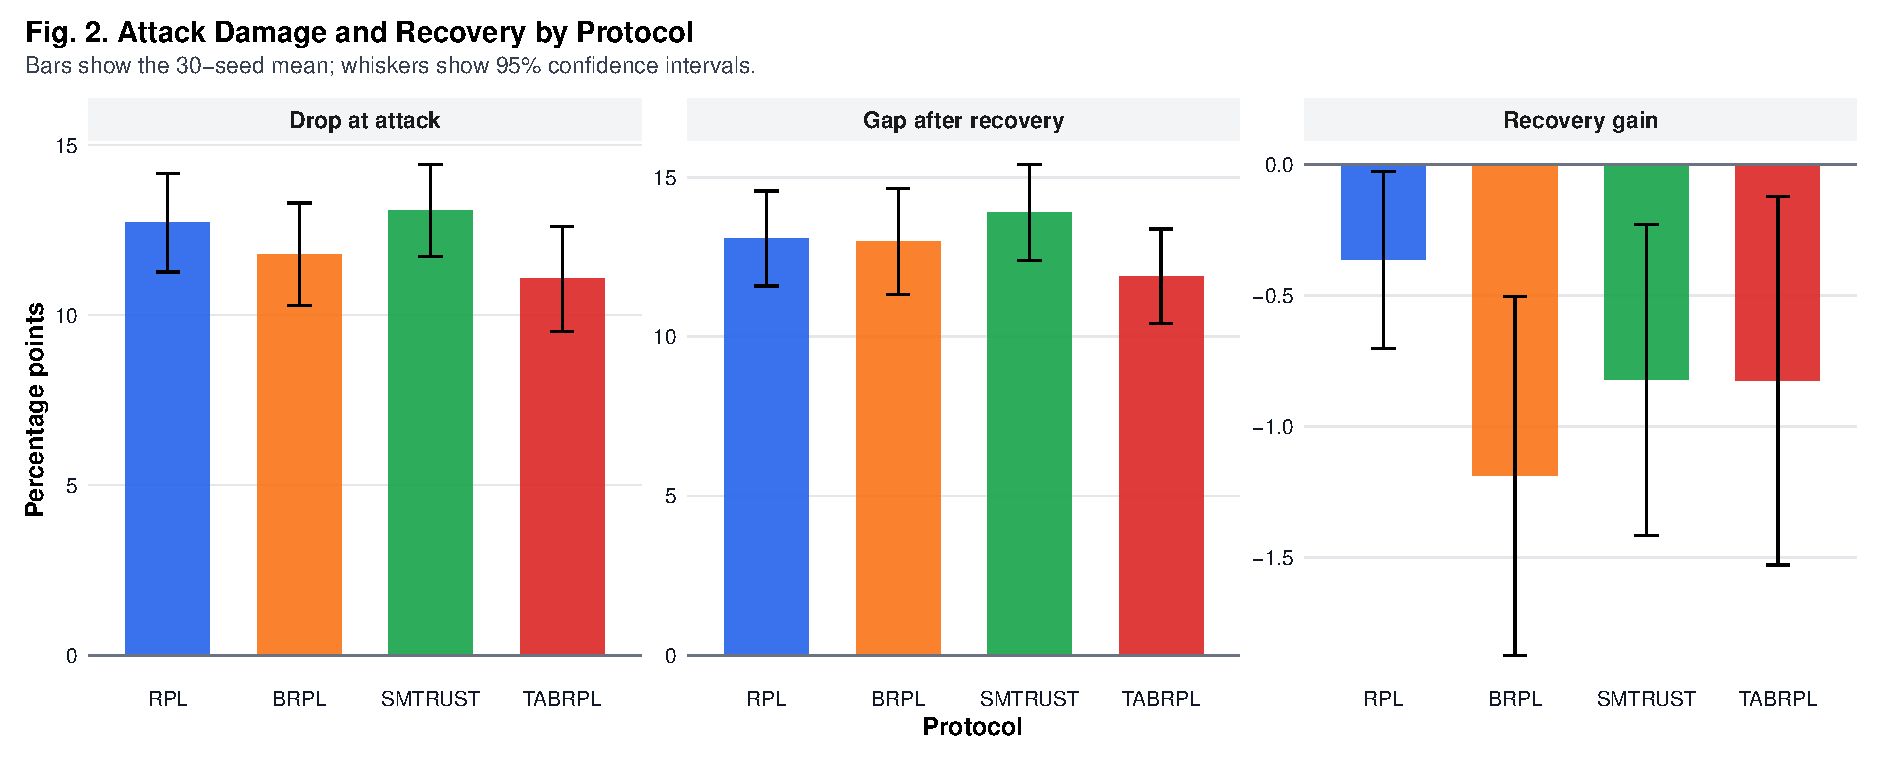
\includegraphics[width=\linewidth]{fig2_resilience_summary.pdf}
  \caption{공격 복원력 요약. TA-BRPL에서는 recovery PDR이 during-attack PDR보다 높게 나타나는
  trust convergence effect가 뚜렷하게 관찰된다.}
  \label{fig:resilience}
\end{figure}

\subsection{Trust Convergence Effect}

TA-BRPL의 recovery PDR(0.9593)은 during-attack PDR(0.9077)보다 높다.
공격자가 recovery 구간에서도 계속 활성 상태임을 고려하면 이는 직관에 반하는 결과처럼 보인다.

그 원인은 150초 주기의 EWMA 업데이트 지연에 있다.
\begin{itemize}
  \item 1차 창(350--500초): EWMA trust가 대략 550 수준까지 하락한다.  
  cost penalty는 적용되지만 아직 parent 후보에서 완전히 제외되지는 않는다.
  \item 2차 창(500--650초): halving decay가 누적되면서 trust가
  $\tau_\text{join}=450$ 이하로 하락한다. 이 시점부터 공격자 노드가 parent 후보 집합에서 제거되기 시작한다.
  \item Recovery 구간(650--900초): 공격자 배제가 충분히 적용되고,
  트래픽이 대안 경로로 재수렴하면서 PDR이 상승한다.
\end{itemize}

이 현상은 전체 30개 seed 중 29개에서 관찰되었으며, 평균 상승폭은 $+5.2$\,pp였다.

반면 SMTrust에서는 이러한 효과가 관찰되지 않는다
(recovery 대비 during 변화량 $-0.05$\,pp).
이는 SMTrust가 공격자 노드를 parent 후보 집합에서 실질적으로 제거하지 못하기 때문이다
(Section~\ref{sec:smtrust}의 TI floor 분석 참조).

\begin{figure}[t]
  \centering
  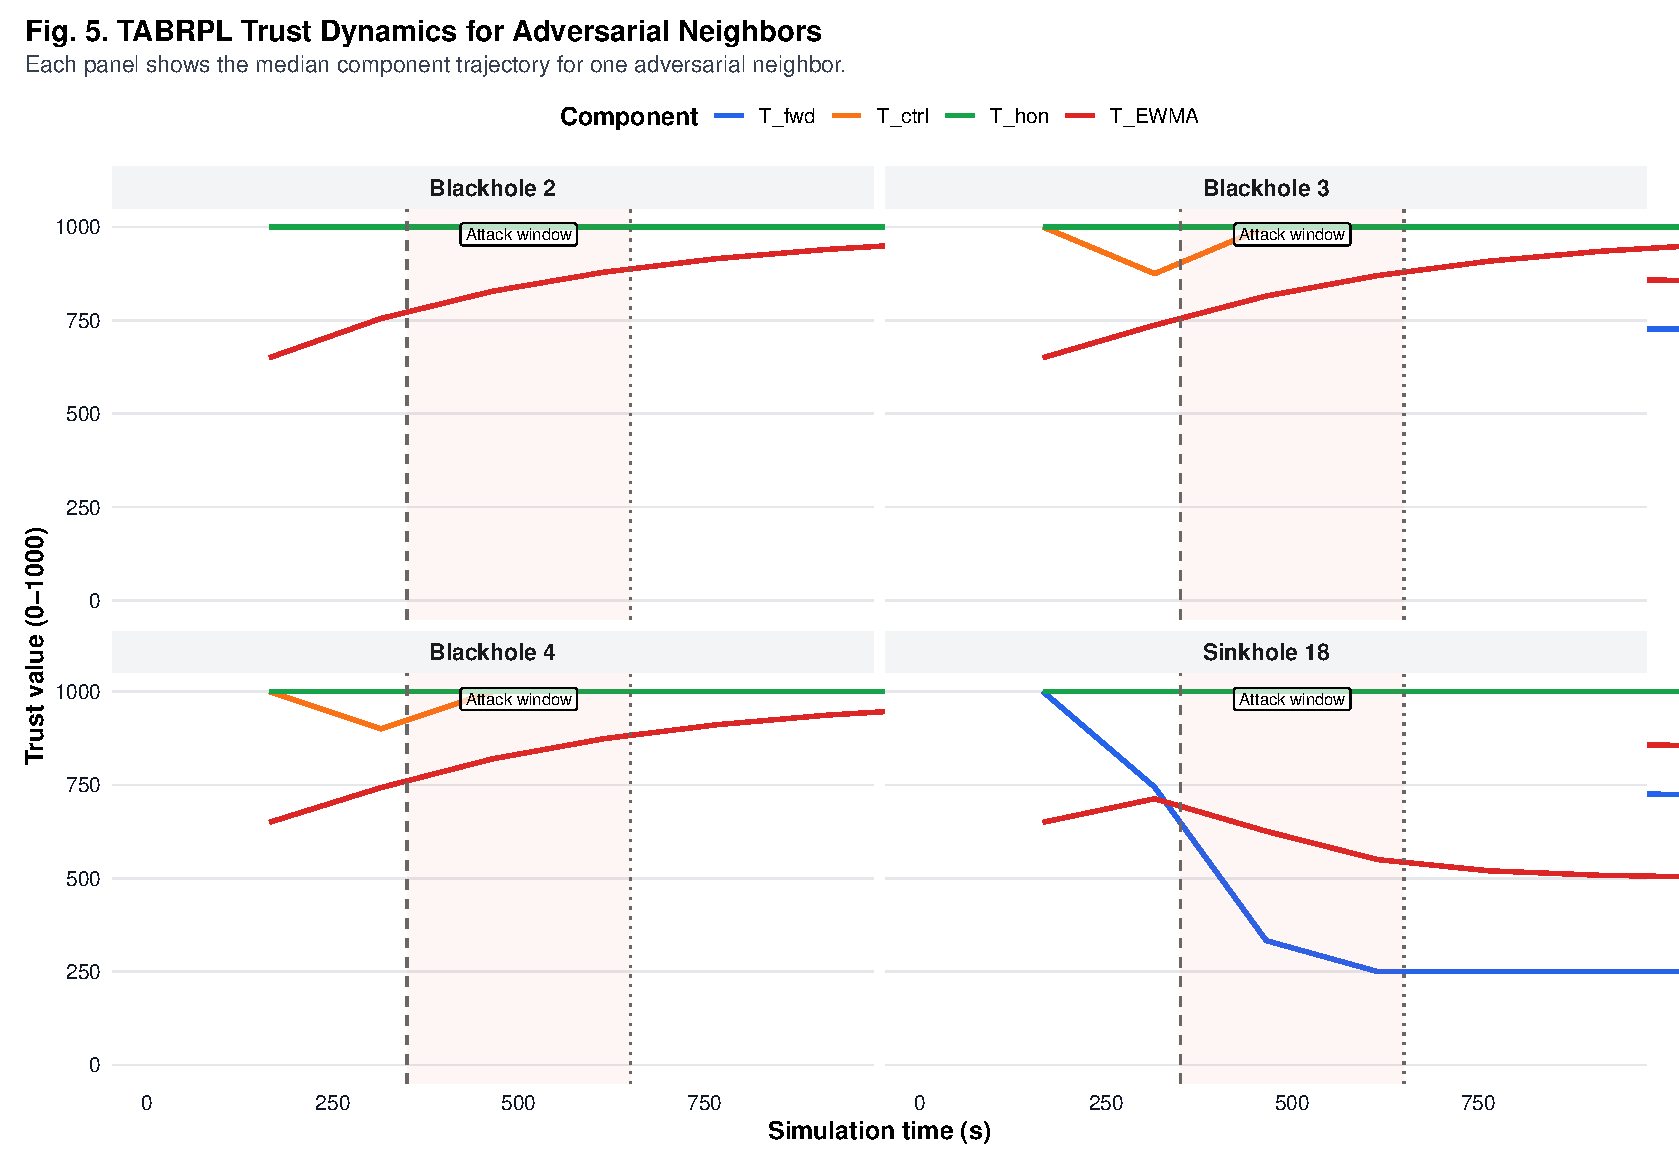
\includegraphics[width=\linewidth]{fig5_trust_trace.pdf}
  \caption{단일 seed에서의 trust trace. 공격자(attacker) 노드의 $T_\text{fwd}$가
  350초 이후 급격히 하락하여 $\tau_\text{join}=0.45$ 아래로 내려가고,
  이후 recovery 구간에서 대안 경로로의 전환이 이루어지는 과정을 보여준다.}
  \label{fig:trust_trace}
\end{figure}

% ============================================================
\section{V2: 오탐(FPR) 실험}
% ============================================================

공격자가 존재하지 않는 환경에서, TA-BRPL이 정상 노드를 부당하게 격리하는지 확인하기 위해
5-seed 실험을 수행하였다. 이때 기존 공격자 노드는 일반 sender로 대체하였다.

\begin{table}[t]
  \centering
  \caption{공격이 없는 환경에서의 PDR (5 seeds)}
  \label{tab:noattack}
  \begin{tabular}{lrrr}
    \toprule
    프로토콜 & Pre & During & Recovery \\
    \midrule
    RPL (no attack)     & 1.0000 & 1.0000 & 1.0000 \\
    BRPL (no attack)    & 1.0000 & 0.9994 & 1.0000 \\
    TA-BRPL (no attack) & 0.9800 & 0.8571 & 0.7886 \\
    \bottomrule
  \end{tabular}
\end{table}

TA-BRPL\_NOATTACK의 during PDR은 0.8571로 비교적 낮게 나타났다.
그러나 이는 전형적인 의미의 FPR(정상 노드의 blacklist)이라기보다,
\textbf{합성 혼잡 버스트(200--300초)로 인해 $T_\text{hon}$이 혼잡 노드에 패널티를 부여한 결과}에 가깝다.
이 해석은 V3 분리 실험(Section~\ref{sec:v3})에서 확인된다.

\begin{figure}[t]
  \centering
  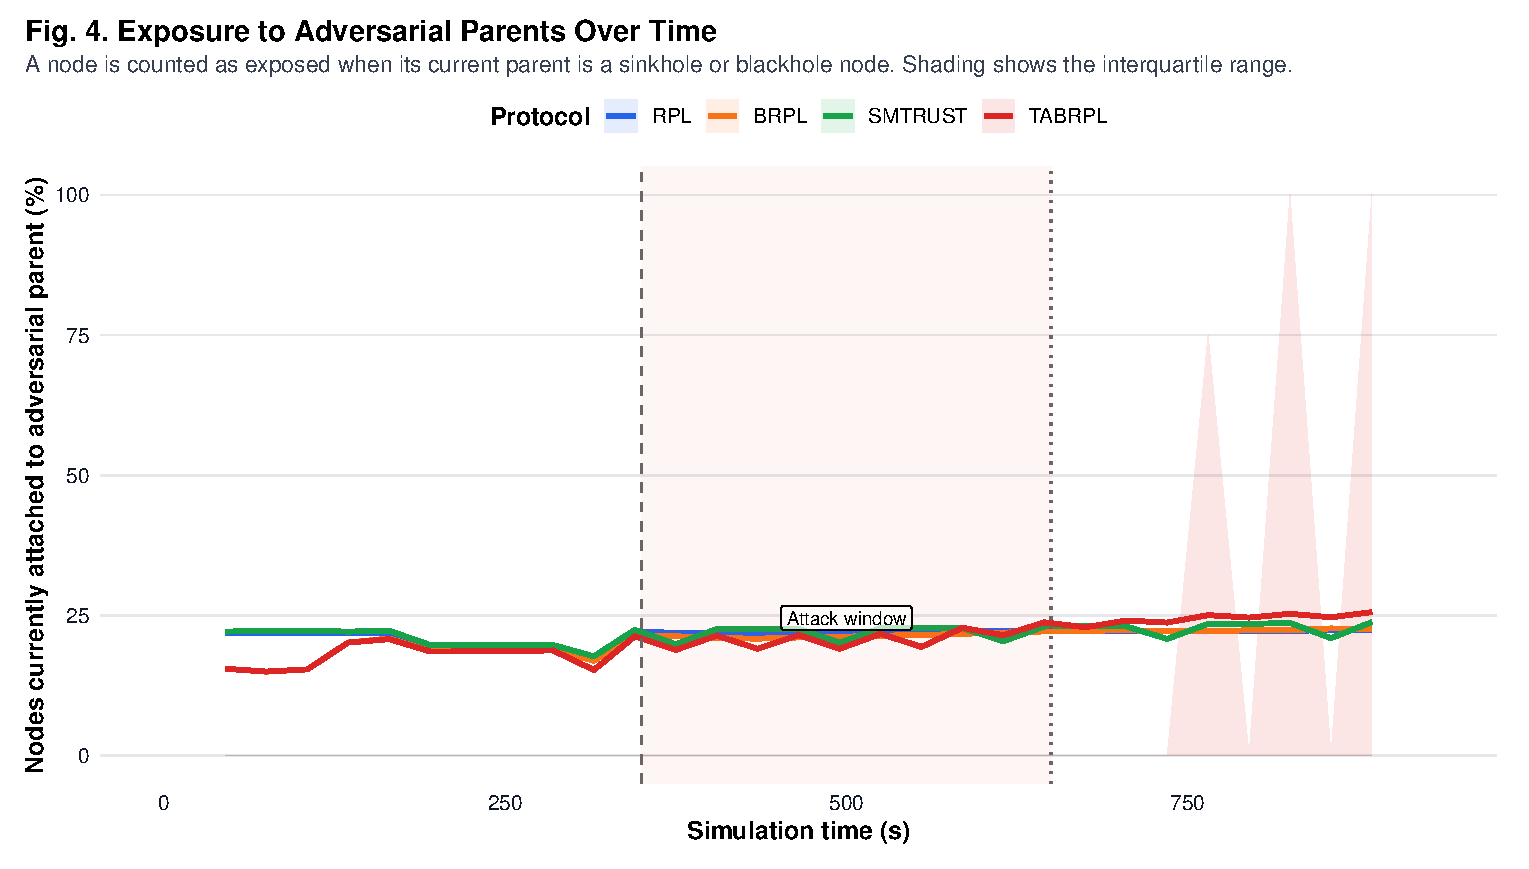
\includegraphics[width=\linewidth]{fig4_route_exposure_timeseries.pdf}
  \caption{공격자 노드를 경유하는 라우트 비율의 시계열(30-seed 평균).
  TA-BRPL은 공격 시작(350초) 이후 가장 빠르게 공격자 노드 노출을 감소시키며,
  recovery 구간에서는 거의 0에 수렴한다.}
  \label{fig:exposure_ts}
\end{figure}

% ============================================================
\section{V3: 혼잡 vs. 공격 분리 실험}
\label{sec:v3}
% ============================================================

TA-BRPL의 핵심 주장인 ``단순 PDR 하락 $\ne$ 공격''을 검증하기 위해,
혼잡과 공격을 각각 독립적으로 on/off한 4개 시나리오를 구성하여 실험하였다.

\begin{table}[t]
  \centering
  \caption{V3 혼잡--공격 분리 실험 결과 (5 seeds, TA-BRPL)}
  \label{tab:v3}
  \begin{tabular}{lllrrr}
    \toprule
    시나리오 & 혼잡 & 공격 & Pre & During & Recovery \\
    \midrule
    C1: Baseline    & \texttimes & \texttimes & 0.961 & 0.793 & 0.875 \\
    C2: 혼잡만      & \checkmark & \texttimes & 0.980 & 0.857 & 0.789 \\
    C3: 공격만      & \texttimes & \checkmark & 0.994 & 0.379 & 0.595 \\
    C4: 혼잡+공격   & \checkmark & \checkmark & 0.999 & 0.417 & 0.353 \\
    \bottomrule
  \end{tabular}
\end{table}

핵심 비교는 \textbf{C2(0.857) $\gg$ C3(0.379)}이다.
혼잡만 존재하는 경우에는 $T_\text{hon}$이 혼잡 노드에 적절한 패널티를 부여하지만,
전체 PDR은 상대적으로 크게 악화되지 않는다. 반면 공격만 존재하는 경우에는
$T_\text{fwd}$가 급락하면서 조기 blacklist가 유도되고, PDR이 크게 하락한다.
이 대비는 ``TA-BRPL이 혼잡과 공격을 구분한다''는 주장의 실험적 근거를 제공한다.

\begin{figure}[t]
  \centering
  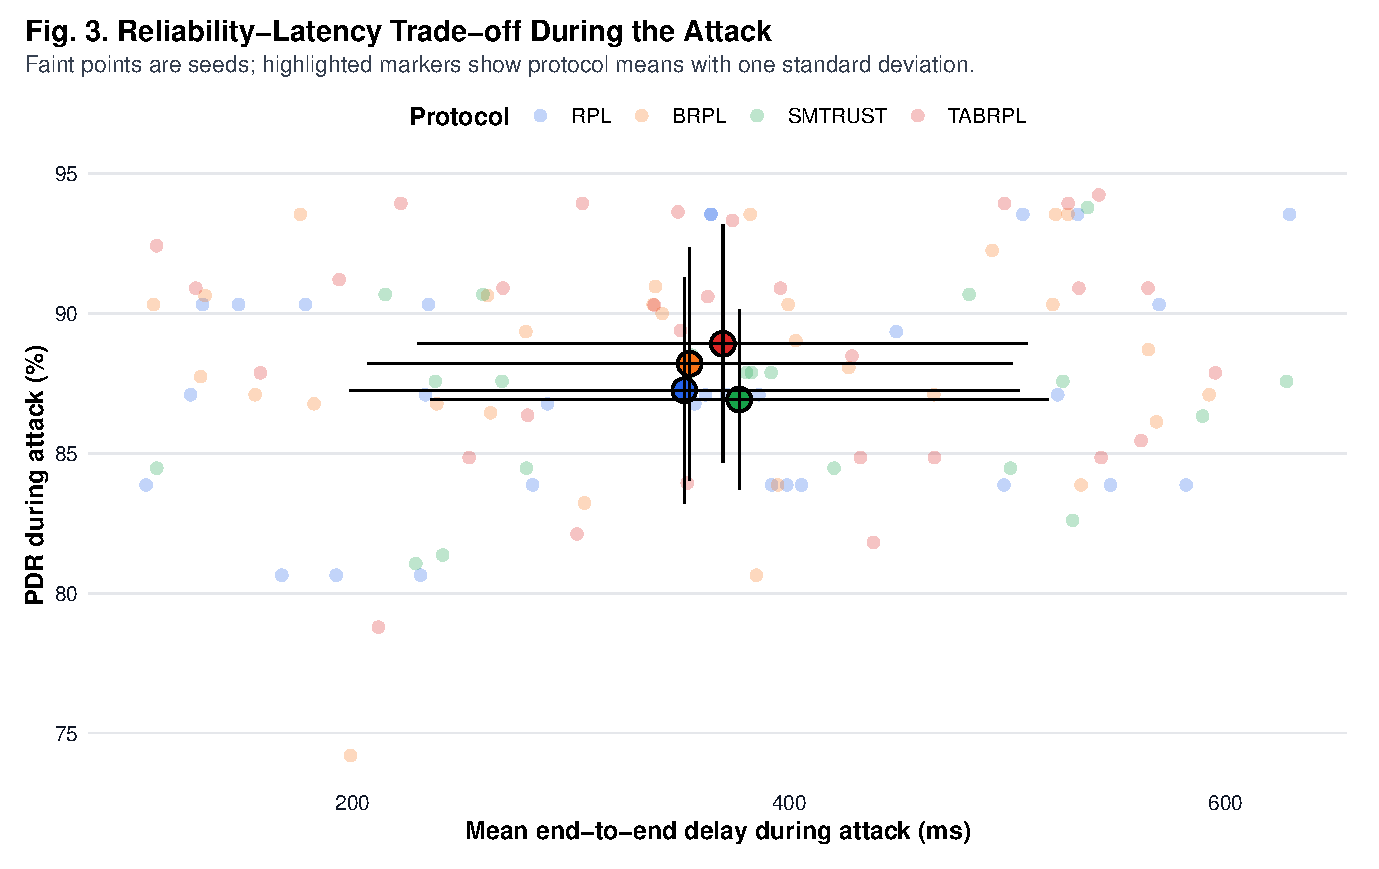
\includegraphics[width=\linewidth]{fig3_attack_tradeoff.pdf}
  \caption{V3 혼잡--공격 분리 실험 결과. C2(혼잡만)와 C3(공격만)의 during PDR 차이가
  뚜렷하게 나타나며, $T_\text{hon}$과 $T_\text{fwd}$가 서로 다른 원인을 탐지함을 보여준다.}
  \label{fig:attack_tradeoff}
\end{figure}

한편, C1(혼잡 없음, 공격 없음)에서도 during PDR이 0.793까지 하락한다.
이는 공격 때문이 아니라, TA-BRPL 자체의 trust penalty 기반 경로 재평가 과정에서
정상 노드에 대해 escape/persistence 패널티가 발동하는 비용으로 해석된다.

% ============================================================
\section{V5: EWMA 파라미터 민감도}
% ============================================================

$\lambda_\downarrow$와 $\lambda_\uparrow$의 선택을 정당화하기 위해,
4개의 변형을 각각 5-seed씩 실험하였다(Table~\ref{tab:lambda}).

\begin{table}[t]
  \centering
  \caption{EWMA $\lambda$ 민감도 분석 (5 seeds)}
  \label{tab:lambda}
  \begin{tabular}{llrr}
    \toprule
    변형 & $(\lambda_\downarrow,\,\lambda_\uparrow)$ & During PDR & Recovery PDR \\
    \midrule
    \textbf{기본값 (TA-BRPL)} & $(0.5,\;0.7)$ & \textbf{0.908} & \textbf{0.959} \\
    LAMBDA\_FAST              & $(0.1,\;0.7)$ & 0.384 & 0.444 \\
    LAMBDA\_SLOW              & $(0.4,\;0.7)$ & 0.474 & 0.490 \\
    LAMBDA\_FAST\_RECOVERY    & $(0.2,\;0.5)$ & 0.517 & 0.561 \\
    LAMBDA\_SLOW\_RECOVERY    & $(0.2,\;0.9)$ & 0.534 & 0.685 \\
    \bottomrule
  \end{tabular}
\end{table}

모든 변형은 기본값보다 현저히 낮은 성능을 보였다. 그 해석은 다음과 같다.
\begin{itemize}
  \item \textbf{LAMBDA\_FAST ($\lambda_\downarrow=0.1$)}: 신규 관찰에 90\%의 가중치를 부여하므로
  EWMA 분산이 급격히 증가하고, 정상 노드도 단일 관찰 창에서 FP blacklist될 수 있다.
  그 결과 during PDR이 0.384까지 하락하여 가장 나쁜 성능을 보였다.
  \item \textbf{LAMBDA\_SLOW ($\lambda_\downarrow=0.4$)}: 이름과 달리 기본값(0.5)보다
  신규 관찰 비중이 더 크므로 오히려 더 반응적이다(60\% vs.\ 50\%).
  따라서 FP 비율이 상승한다.
  \item \textbf{FAST/SLOW\_RECOVERY}: 두 변형 모두 $\lambda_\downarrow=0.2$를 사용하므로
  이미 과반응 영역에 진입한 상태다. 따라서 회복 속도의 차이보다 공격 중 FP 증가의 영향이 더 크게 나타난다.
\end{itemize}

결론적으로, $\lambda_\downarrow=0.5$는 공격 반응성과 EWMA 안정성 사이의 균형점으로 해석된다.
특히 $\lambda_\downarrow < 0.5$인 경우에는 분산이 과도하게 증가하여 성능 저하를 초래한다.

% ============================================================
\section{V6: 임계값 민감도}
% ============================================================

$(\tau_\text{warn}, \tau_\text{join}, \tau_\text{black})$의 선택을 정당화하기 위해,
3개 변형을 각각 5-seed씩 실험하였다(Table~\ref{tab:thresh}).

\begin{table}[t]
  \centering
  \caption{임계값 민감도 분석 (5 seeds). 기본값: $(0.70,\;0.45,\;0.25)$}
  \label{tab:thresh}
  \begin{tabular}{lp{2.2cm}rr}
    \toprule
    변형 & $(\tau_w,\;\tau_j,\;\tau_b)$ & Pre PDR & During PDR \\
    \midrule
    \textbf{기본값} & $(0.70,\;0.45,\;0.25)$ & 0.999 & \textbf{0.908} \\
    THRESH\_STRICT  & $(0.80,\;0.60,\;0.40)$ & 0.914 & 0.586 \\
    THRESH\_RELAXED & $(0.70,\;0.50,\;0.30)$ & 0.993 & 0.494 \\
    THRESH\_JOINLOW & $(0.75,\;0.40,\;0.25)$ & 0.999 & 0.750 \\
    \bottomrule
  \end{tabular}
\end{table}

\begin{itemize}
  \item \textbf{THRESH\_STRICT}: $\tau_\text{join}=0.60$이 지나치게 높아,
  네트워크 수렴 과정에서 자연스럽게 forwarding rate가 낮은 정상 노드까지
  후보에서 제외된다. 그 결과 pre PDR이 이미 0.914까지 하락한다.
  \item \textbf{THRESH\_RELAXED}: $\tau_\text{join}=0.50$으로 상승하면
  trust가 $[0.45,0.50)$ 구간에 있는 노드가 더 오래 후보로 남게 되어 탐지가 지연된다.
  결과적으로 during PDR이 0.494로 크게 악화된다.
  \item \textbf{THRESH\_JOINLOW}: $\tau_\text{join}=0.40$으로 낮추면
  suspect 구간이 넓어지고(0.40$\sim$0.75), 배제 전 패널티 기간이 길어진다.
  다만 완전 배제까지의 시간이 증가하여 during PDR은 0.750 수준에 머문다.
\end{itemize}

결론적으로 기본값 $(0.70, 0.45, 0.25)$는 EWMA 파라미터와 함께 설계된
실질적 최적점으로 해석된다. 특히 $\tau_\text{warn} - \tau_\text{join} \ge 0.20$의
간격을 확보하는 것이 중요하다.

% ============================================================
\section{절제 실험: 3성분 필요성 검증}
% ============================================================

각 trust 성분의 기여를 독립적으로 확인하기 위해,
단일 성분 또는 2성분 변형을 각각 5-seed씩 실험하였다(Table~\ref{tab:ablation}).

\begin{table}[t]
  \centering
  \caption{성분 절제 실험 결과 (5 seeds)}
  \label{tab:ablation}
  \begin{tabular}{lllrrr}
    \toprule
    변형 & 성분 & Pre & During & Recovery \\
    \midrule
    TA-BRPL (전체) & $T_f + T_c + T_h$ & 0.999 & \textbf{0.908} & \textbf{0.959} \\
    FWD+CTRL       & $T_f + T_c$        & 0.926 & 0.660 & 0.516 \\
    FWD only       & $T_f$ only         & 0.898 & 0.719 & 0.731 \\
    \midrule
    RPL (기준)     & 없음               & 1.000 & 0.876 & 0.875 \\
    \bottomrule
  \end{tabular}
\end{table}

흥미롭게도, \textbf{두 변형 모두 RPL보다 낮은 성능을 보였다}.
예를 들어 FWD only의 during PDR(0.719)은 RPL의 during PDR(0.876)보다 낮다.

그 이유는 다음과 같다.
\begin{enumerate}
  \item FWD only에서는 pre PDR이 이미 0.898로 하락한다.  
  이는 네트워크 수렴 초기의 자연스러운 forwarding rate 저하가 FP blacklist로 이어지기 때문이다.
  \item FWD+CTRL에서는 pre PDR이 0.926으로 다소 개선되지만,
  DIO trickle 정착 구간에서 DIO 빈도 이상 역시 FP를 추가로 유발한다.
  \item $T_\text{hon}$이 있어야 이러한 FP가 억제된다.  
  혼잡 구간에서 정상 노드의 $T_\text{hon} \approx 1.0$이 EWMA를 안정화하여,
  pre-attack FP를 줄이는 역할을 한다.
\end{enumerate}

즉, 세 trust 성분은 선택적으로 더하는 부가 요소가 아니라,
\textbf{함께 사용될 때에만 의미를 갖는 상보적 구성}으로 해석할 수 있다.
특히 $T_\text{hon}$이 없으면 $T_\text{fwd}$ 단독 사용은 오히려 RPL보다 더 나쁜 결과를 낳는다.

\begin{figure}[t]
  \centering
  
\includegraphics[width=\linewidth]{fig6_churn_hotspots.pdf}
  \caption{Parent churn 핫스팟 분포. FWD-only 변형에서는 공격자 인근 노드의
  parent 교체 빈도가 급증하며, $T_\text{hon}$을 추가하면 이 현상이 억제된다.}
  \label{fig:churn}
\end{figure}

% ============================================================
\section{손실률 로버스트니스}
% ============================================================

UDGM의 \texttt{success\_ratio}를 각각 0.9(10\% 손실), 0.8(20\% 손실)로 낮추어
링크 손실 환경에서의 robustness를 확인하였다(5 seeds).

\begin{table}[t]
  \centering
  \caption{링크 손실률별 during-attack PDR (5 seeds)}
  \label{tab:loss}
  \begin{tabular}{lrrr}
    \toprule
    프로토콜 & 손실 0\% & 손실 10\% & 손실 20\% \\
    \midrule
    RPL      & 0.876 & 0.803 ($-8.3$\,pp)  & 0.761 ($-13.1$\,pp) \\
    BRPL     & 0.851 & 0.838 ($-1.5$\,pp)  & 0.730 ($-14.2$\,pp) \\
    TA-BRPL  & 0.908 & \textcolor{red}{0.540 ($-40.5$\,pp)} & \textcolor{red}{0.512 ($-43.7$\,pp)} \\
    \bottomrule
  \end{tabular}
\end{table}

TA-BRPL은 링크 손실에 훨씬 민감하게 반응하였다.
그 원인은 링크 손실이 증가하면 $F_{ij}$는 감소하지만 $S_{ij}$는 유지되므로,
결과적으로 $T_\text{fwd}$가 하락하고 정상 릴레이 노드까지 FP blacklist될 수 있기 때문이다.

이는 현재 실험에서 가장 큰 실용적 한계다.
실제 배포 환경에서는 링크 품질 보정 팩터를 $T_\text{fwd}$에 반영하거나,
손실률이 높은 환경에서 $\tau_\text{black}$을 더 보수적으로 조정할 필요가 있다.

% ============================================================
\section{\texttt{parse\_results.py} 버그 수정}
% ============================================================

실험 결과 분석 중 두 개의 심각한 파싱 버그가 발견되었고, 이후 수정되었다.

\textbf{버그 1 (CSV,RX offset 오류)}: \texttt{CSV,RX} 로그 형식은
\texttt{CSV,RX,node=1,<src\_ip>,<seq>,...}이며,
comma split 결과는 \texttt{parts=[CSV,RX,node=1,...]}가 된다.
기존 코드는 \texttt{parts[1].startswith("node=")}를 검사했는데,
이는 \texttt{"RX".startswith(...)}와 동일하여 항상 False가 된다.
그 결과 offset이 0으로 고정되었고,
이후 \texttt{int("node=1")}에서 \texttt{ValueError}가 발생하여
모든 RX 레코드가 무시되었다.
즉, 모든 프로토콜의 PDR이 0.0으로 잘못 출력되는 문제가 있었다.
수정 후에는 \texttt{parts[2].startswith("node=")}로 변경하였다.

\textbf{버그 2 (seq-only PDR 매칭)}:
기존 PDR 계산은
$|\{\text{tx seq}\} \cap \{\text{rx seq}\}| / |\{\text{tx seq}\}|$
형태로 이루어져, node ID 없이 seq 번호만 매칭하였다.
그러나 각 sender는 seq 카운터를 독립적으로 1부터 시작하므로,
seq 번호는 전역적으로 유일하지 않다.
예를 들어 node 5의 seq=1과 node 7의 seq=1은 모두 동일한 집합 원소 \{1\}로 처리되어,
둘 중 하나만 수신되어도 ``둘 다 수신됨''으로 계산될 수 있었다.
그 결과 모든 프로토콜의 PDR이 1.0으로 잘못 출력되었다.
수정 후에는 \texttt{set(zip(node\_id, seq))} 형태의 쌍으로 매칭하도록 변경하였다.

% ============================================================
\section{전체 파라미터 목록}
% ============================================================

\begin{table}[t]
  \centering
  \caption{TA-BRPL 주요 파라미터 (\texttt{project-conf.h} 기준)}
  \label{tab:params}
  \begin{tabular}{lll}
    \toprule
    파라미터 & 심벌 & 기본값 \\
    \midrule
    \multicolumn{3}{l}{\textit{임계값}} \\
    Warn 임계값       & $\tau_\text{warn}$    & 700 \\
    Join 임계값       & $\tau_\text{join}$    & 450 \\
    Blacklist 임계값  & $\tau_\text{black}$   & 250 \\
    초기 신뢰         & $T_\text{init}$       & 500 \\
    \midrule
    \multicolumn{3}{l}{\textit{EWMA}} \\
    감소 람다         & $\lambda_\downarrow$  & 0.5 \\
    정상 람다         & $\lambda_\uparrow$    & 0.7 \\
    업데이트 주기     & $\Delta t$            & 150s \\
    \midrule
    \multicolumn{3}{l}{\textit{가중치}} \\
    $T_\text{fwd}$ 가중치   & $w_f$      & 5 \\
    $T_\text{ctrl}$ 가중치  & $w_c$      & 3 \\
    $T_\text{hon}$ 가중치   & $w_h$      & 2 \\
    Laplace $\alpha$        & $\alpha$   & 1 \\
    Laplace $\beta$         & $\beta$    & 1 \\
    Rank 이상 가중치        & $w_1$      & 5 \\
    DIO 이상 가중치         & $w_2$      & 3 \\
    Version 이상 가중치     & $w_3$      & 2 \\
    \midrule
    \multicolumn{3}{l}{\textit{Blacklist / 회복}} \\
    격리 기간               & $t_\text{bl}$     & 120s \\
    해제 후 복원 신뢰       & $T_\text{rst}$    & 450 \\
    해제 cooldown           & $t_\text{cool}$   & 120s \\
    해제 초기 패널티 배율   & $P_\text{rel}$    & $1.6\times$ \\
    지속 패널티 창          & $t_\text{per}$    & 120s \\
    지속 패널티 step        & $\Delta P$        & 250 \\
    지속 패널티 최대값      & $P_\text{max}$    & $2.6\times$ \\
    Escape 발동 시간        & $t_\text{esc}$    & 180s \\
    Escape 패널티 배율      & $P_\text{esc}$    & $3.2\times$ \\
    Escape 신뢰 임계값      & $\tau_\text{esc}$ & 700 \\
    \midrule
    \multicolumn{3}{l}{\textit{실험 환경}} \\
    토폴로지     & -- & GRID $6\times6$, 36 노드 \\
    공격자       & -- & Blackhole $\times3$ + Sinkhole $\times1$ \\
    Seed 수      & -- & 30 \\
    송신 주기    & -- & 30s \\
    시뮬레이션   & -- & 900s \\
    \bottomrule
  \end{tabular}
\end{table}

% ============================================================
\section{구현상 한계}
% ============================================================

\textbf{L1 정적 토폴로지}: 모든 실험은 고정 GRID 토폴로지에서 수행되었다.
이동성이 있는 환경에서는 $T_\text{fwd}$의 overhearing 범위 이탈로 인해
FP가 증가할 가능성이 있다.

\textbf{L2 무손실 링크}: 기본 실험은 UDGM \texttt{success\_ratio=1.0} 환경에서 수행되었다.
그러나 실제 IEEE 802.15.4 환경에서는 PRR이 대략 0.7--0.9 수준일 수 있으므로,
이 경우 $T_\text{fwd}$ 기반 FP가 크게 증가할 수 있다.
따라서 링크 품질 보정 항의 도입이 필요하다.

\textbf{L3 제한된 공격 유형}: 현재 평가는 Blackhole + rank sinkhole에 한정되어 있다.
Colluding sinkhole, version attack, Sybil attack 등은 아직 평가하지 않았다.

\textbf{L4 도청 불완전성}: IP 레이어 도청 훅은 MAC 필터링으로 폐기된 패킷을 감지하지 못한다.
현재 UDGM에서는 모든 프레임이 IP 레이어까지 전달되므로 이 문제가 가려져 있다.

\textbf{L5 SMTrust DIO 확장}: TMRT 성분은 비표준 ICMPv6 옵션(0xFE, 0x02)을 사용한다.
따라서 RFC 호환성이 없다.

\textbf{L6 부동소수점}: 현재 Cooja 구현에서는 기하평균 계산에 glibc의
\texttt{pow()}를 사용한다. 실제 MCU(Cortex-M0+) 배포를 고려한다면,
정수 기반 lookup table 방식으로 대체할 필요가 있다.

\end{document}